In order to structure the design process, several design aspects were separated to facilitate a structured approach to iterating over the design. The goal is to find a design that complies with the requirements as given in Section \ref{sec:reqbreak}. This is done by iterating over the design space,  choosing a design concept, containing a combination of an aerodynamic shape, trajectory, \gls{tps}, inflation structure and control system and analysing its performance. After that, the analysis of the concept is used to assess possible points of improvement if the requirements are still not met. This is done until all requirements are met.


The aerodynamic shape is chosen such that certain aerodynamic properties are achieved. This is largely done by optimisation since this allows a high fidelity in design optimisation objectives and constraints. When a suitable design is chosen, the resulting aerodynamic performance is used in determining a trajectory that complies with the initial and final velocity and height requirements. This is done by choosing a bank angle profile. The trajectory data containing velocity, density, Mach number and dynamic pressure is used for the inflation structure sizing, \gls{tps} lay-up and control system mass estimation. The shape and maximum dynamic pressure in the trajectory is used in determining the inflation structure, for which a representative truss structure is used to size the structure and obtain its mass. The trajectory data is used to calculate the heat flux into the system, which in turn amounts to a temperature distribution through the structure and through time. The lay-up is then iterated until no layer temperature exceeds its maximum temperature while having the smallest thickness possible such that the \gls{tps} has the lowest possible mass. The control system mass is finally estimated using the aerodynamic moment coefficients and required trajectory.

When the technical analysis of the concept is done, the iteration is completed by analysing the results and assessing points where improvement can be made. When not all requirements are met, changes have to be made tot he design. Several problems have been identified during the design phase:
\begin{itemize}
	\item In the case the temperature in the different \gls{tps} layers become too high, even for high thicknesses, the orbit needs to be changed to facilitate a lower maximum dynamic pressure. This can be done by choosing the lowest point of atmospheric entry higher such that the density is lower. If achieving orbit at this higher point is not possible with the current aerodynamic design, the drag coefficient is to be increased to allow the same deceleration at lower dynamic pressures.
	
	\item If the thermal protection system mass or inflation structure mass makes the total design exceed the mass requirement, also the maximum dynamic pressure is to be decreased such that physical loads on the structure and thermal loads on the \gls{tps} are decreased.
	
	\item If bank angle control does not perform well enough to allow a trajectory that satisfies the requirements, the lift over drag ratio can be increased to allow more freedom in trajectory choice.
	
	
\end{itemize}

The iteration strategy is visualised as a flow-chart in Figure \ref{fig:iterativedesignflowchart}. In this figure the solid lines represent design information flowing towards the areas that still need analysis. The dotted lines represent feedback information, which is needed when a requirement is violated. If 



For the new shape, the trajectory is determined using a fixed \gls{sym:alpha}. The aerocapture phase is then tuned to a 


\begin{figure}[h!]
		\vspace{-1cm}
		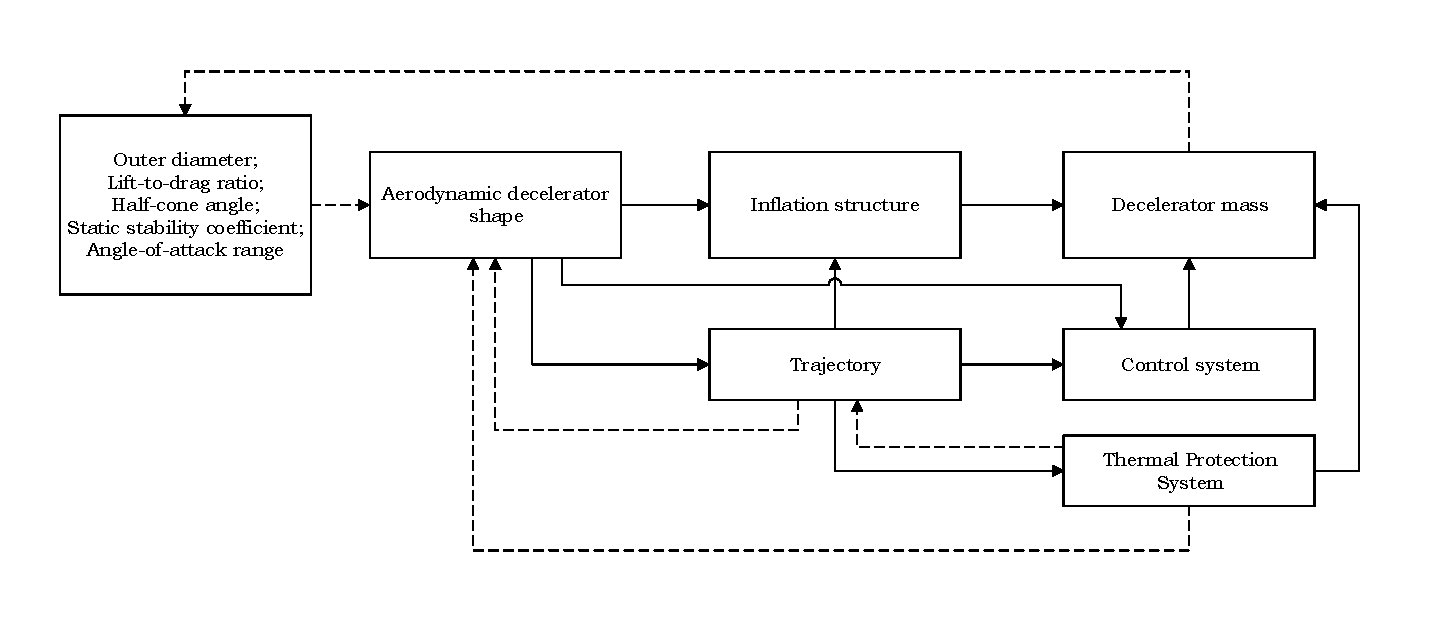
\includegraphics[width=0.96\textwidth]{./Figure/DesignIterationPhilosophy.pdf}
		\vspace{-2.3cm}
		\caption{The iterative design process flowchart}
		\label{fig:iterativedesignflowchart}
\end{figure}